\subsection{溶剂的选择和水溶液的结构}
从溶液中生长晶体除了最常用的溶剂——水以外,还可使用其他溶剂,如重水、乙醇、丙醇、氯仿、四氯化碳、苯、甲苯、二甲苯等。有时还应用两种或多种溶剂混合物,如乙醇—水、乙醇—甲苯、甲醇—甘油等。

选择溶剂时,一般需要综合考虑溶剂的性质、经济和安全等方面的因素。具体地说需要注意以下几个问题:
\begin{enumerate}[(1)]\itemsep -0.5ex
\item 对溶质要有足够大的溶解度(一般要求在10---60\%的范围内)。这里有一条“相似相溶"规律,即物质易溶于化学上与其相似的溶剂中。例如,一些极性大的盐类易溶于水,非极性溶质(如蒽)在非极性溶剂(如苯)中的溶解度要比在极性溶剂(如水)中大得多。
\item 合适的溶解度温度系数。溶剂对溶质最好有正的溶解度温度系数。但也不宜过大,因为后者要求十分精密的温度控制。
\item 有利于晶体生长。溶质和溶剂之间在结构上的关系对晶体生长有一定的影响。例如联苯酰[$\rm (C_6H_5CO)_2$]在乙醇中有较大的溶解度,但不能从其溶液中结晶,而能从结构上与其有相似之处的苯$\rm C_6H_6$中结晶。这表明从溶液中生长晶体的难易程度,可能取决于溶质在晶体中和在溶液中缔合情况的相似性。这里还涉及到溶质和溶剂的相互作用同题。另外,选择溶剂时还需注意使溶质在该溶剂中结晶时呈现有利的晶癖。如使结晶呈板状而不是针状,这一点在工业结晶中十分重要。
\item 纯度和稳定性要高。溶剂应无色透明和尽可能的纯净,在化学上则要稳定、不分解、不氧化也不与溶质起化学作用及对容器材料无腐蚀性等。如使用有机溶剂,还需注意选择与其入起作用的密封材料等。
\item 其他要求,如溶剂的挥发性要低、粘度和毒性要小、价格要便宜等。
\end{enumerate}

选取同时满足上述要求的溶剂是不容易的,有时需要在溶剂中加人一些辅助剂或使用混合溶剂来改善某些性质(如改变溶解度和粘度等)。常用溶剂的一些性质列于表3.3中。

(表3.3)
%TODO: 表3.3

水是一种很理想的溶剂。水的溶解能力很强,能溶解许多无机和有机盐类,而且容易通过温度变化和除去水的方法来控制溶液的过饱和度;水的稳定性好、粘度小、无害、加上水在自然界的大量存在和易于提纯等原因,使得水成为所有溶剂中最重要、利用最为广泛的溶剂。

水具有许多不同寻常的性质,如高熔点(与有关的氢化物相比)、高热导率、高介电常量和表面张力、低的熔化熵以及4℃ 时具有最大密度等特性,这些都说明了液态水也是有一定结构的。

众所周知,在水的结构中,水分子由氢键联接起来形成四面体堆积,中间有许多空隙。而对于水来说,在短程有序的意义上,可以把水看作为是被分子热运动破坏了的、但仍保有局部冰的构造这样一种结构。这就是说,水在近程内,每个原子的周围乃保留以四面体方式配置的松散的局部的氢键。所以在水中存在着由氢键联接起来的、具有类似构造的水分子集团,但寿命很短(约 $\rm 10^{-11}s$)。在重水中,由于氘键比普通氢键牢固,因此其中冰骨架的成分要比普通水中多。

\begin{figure}[htb]
 \centering
 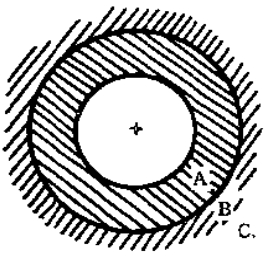
\includegraphics[width=0.4\textwidth]{fig/cp03/img3.12.jpg}
 \caption{水合离子模型。}
\end{figure}
% 图3.12

溶质在水中的存在,显著地改变了液体的性质。例如在电解质的水溶液中,离子是水合的。由于离子的库仑力作用,使水的氢键结构受到局部破坏,并将水分子吸引到自己周围,形成水合离子。根据Frank的水合离子模型(图3.12),包围阳离子的水分子分成A,B,C三层。在A层,包围阳离子的是一些由取向的水分子偶极形成的牢固的水合层,称为“第一级水合球”[也称为内配位球(inner co-ordination sphere)或近程水合(close hydration)]。在该层内,由于离子和水分子的相互作用,水分子不能移动。 但离子的静电作用还能超出A区,形成范围大得多的“第二级水合球"也称为外配位球[(outer co-ordination sphere)或远程水合(distant hydration)](图3 .12中的B区),其中包含的水分子是松散地结合起来的,但没有一定的取向。在c区中,水分子基本上没有受到离子的干扰,只存在水分子之间的相互作用,保持着水的结构。 B 区的情况则是由于A区和C区中两种不同的相互作用所造成的。 对一价的离子,通常有4个分子形成牢固的水合层。对高价离子(如$\rm Cr^{3+}$,$\rm Fe^{3+}$,$\rm Al^{3+}$),第一级水合球则有6个水分子,其水合离子形式为$\rm M(H_2O)_6^{3+}$,水合氢离子$\rm H_3O^+$常以$\rm H_3O(H_2O)^{3+}$形式存在。在水溶液中,离子对晶体生长的影响都和离子的水合有关(参阅3.4.2节)。

在重水溶液中,离子也是水合的,但由于在水合过程中,破坏重水中的氘键要比破坏水中的氢键消耗更多的能量,因此大多数盐类在重水中的溶解度要比在普通水中的溶解度小。磷酸盐是个例外(如$\rm KD_2PO_2$在$\rm D_2O$中的溶解度大于$\rm KH_2PO_2$在$\rm H_2O$中的溶解度),看来这与在磷酸根离子和重水之间形成更加牢固的氘键有关。

上述可见,在溶液中由于存在着离子和溶剂的相互作用(包括溶剂络合物的形成),情况变得较为复杂,有一些问题至今仍未得到解决。

过饱和溶液的结构要比饱和和不饱和溶液更复杂些。不少科学工作者试图通过研究溶液中各种物理性质对浓度的依赖关系来寻找过饱和溶液的特征,但没有取得预期的结果。在许多物质的浓度-性质曲线上,平衡饱和点并未出现不连续性。但实验发现了另一些重要的现象,如将柠檬酸过饱和水溶液恒温静置,在底部区域则会出现浓度梯度。这一现象表明,溶液中存在柠檬酸分子集团,这些分子集团是紧密堆积的柠檬酸分子依靠氢键结合起来的,密度比水的大,这样的体系在热力学上是不稳定的。因此经过一定时间后,在底部出现分层。

在过饱和度很大的酒石酸钾钠(KNT)溶液中,晶体生长异常迅速,这也可能是由于在该溶液中存在由氢键结合起来的KNT分子集团,构成了较大的生长基元,向KNT晶体上堆积的缘故。 

由此可见,开展溶液结构方面的研究,对于了解从溶液中生长晶体的机制是很重要的。目前,关于这一领域的研究仍相当活跃。